\section{Symmetric (secret-key) Crypto}
\subsection{Definition}
\begin{itemize}
  \item A \textbf{cryptosystem} is a triple $(G,E,D)$ of algorithms for key generation, encryption and decryption
  \begin{itemize}
  	\item $G$ \textbf{algorithm for generating keys}:
    \begin{itemize}
  		\item A probabilitstic algorithm
  		\item Takes no input and always outputs a key $K \in \mathcal K$
  		\item It outputs a key space $\mathcal K$ 
    \end{itemize}
  	\item $E$ \textbf{algorithm for encryption}:
    \begin{itemize}
  		\item Takes as input $K$ and $x \in \mathcal P$
  		\item Produces output $E_K(x) \in \mathcal C$
  		\item May be probabilistic
    \end{itemize}
  	\item $D$ \textbf{algorithm for decryption}:
    \begin{itemize}
  		\item Takes as input $K$ and $y \in \mathcal C$
  		\item Produces as output $D_K(y) \in \mathcal P$
  		\item Allowed to be probabilistic but mostly deterministic
    \end{itemize}
  \end{itemize}
  \item A \textbf{symmetric cryptosystem} is where the information you needed to encrypt is the same as what your trying to encrypt
  \item For a symmetric system, there are 3 finite sets given:
  \begin{itemize}
  	\item The key space $\mathcal K$
  	\item The plaintext space $\mathcal P$
  	\item The ciphertext space $\mathcal C$  
  \end{itemize}
  \item It is required for any cryptosystem that for any key output correct decryption is possible
  \begin{itemize}
  	\item i.e. it holds that for any $x \in P, x = D_K(E_K(x))$
  \end{itemize}
\end{itemize}

\subsection{Attacks}
\begin{itemize}
  \item The adversary is thought of as a probabilistic algorithm $A$
  \begin{itemize}
  	\item The data the adversary obtains is modeled as an oracle $O$
  	\item At any time $A$ may call the oracle and obtain an answer
  \end{itemize}

  \item Different form of attacks can be modeled as below where $K$ is chosen from $G$ and is fixed:
  \begin{itemize}
  	\item \textbf{Ciphertext Only Attack:}
    \begin{itemize}
  		\item Some plaintext distribution $D$ is fixed and the algorithm $A$ may depend on $D$
  		\item Each time $A$ calls the oracle it will return $E_K(x)$ where $x$ is chosen according to $D$
    \end{itemize}
  	\item \textbf{Known Plaintext Attack:}
    \begin{itemize}
  		\item A plaintext distribution $D$ is fixed
  		\item The algorithm might depend on $D$
  		\item Each time $A$ calls the oracle it will return $x, E_K(x)$ where $x$ is chosen according to $D$
  		\item Models cases where the adversary can guess with good probability what part of the plaintext is
    \end{itemize}
  	\item \textbf{Chosen Plaintext Attack:}
    \begin{itemize}
  		\item $A$ can call the oracle giving it any input $x \in \mathcal P$ as input
  		\item The oracle returns $E_K(x)$
  		\item Models cases where the adversary can influence the sender into sending some message of the adversary's choice
    \end{itemize}
  	\item \textbf{Chosen Ciphertext Attacks:}
    \begin{itemize}
  		\item $A$ can call the oracle giving it any $y \in \mathcal C$ as input
  		\item The oracle returns $D_K(y)$
  		\item Models cases where the adversary sends a ciphertext he constructed to the receiver and when monitoring the receiver's behavior he might get new information
    \end{itemize}
  \end{itemize}
  \item When $A$ stops it outputs some result
  \begin{itemize}
  	\item In the best case for the adversary it is the secret key
  	\item Adversaries with much less ambitious goals might also be considered
    \begin{itemize}
  		\item e.g. computing some partial information on an unknown plaintext
    \end{itemize}
  \end{itemize}
  \item The shift cipher can be attacked using exhaustive key search or frequency analysis for a ciphertext only attack
\end{itemize}

\subsection{DES blockcipher}
\begin{figure}[H]
	\centering
	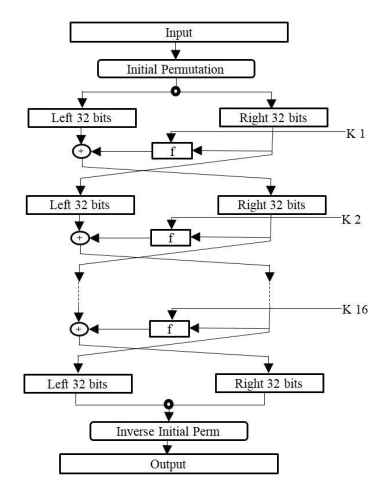
\includegraphics[width=220pt]{img/symmetric_cryptosystems/des_structure}
	\caption{Structure of DES}
\end{figure}
\begin{itemize}
  \item A \textbf{Feistel cipher} encryption consists of repeating some computation a number of times
  \begin{itemize}
  	\item One such computation is called a round and the number of rounds is denoted $n$
  	\item There is an algorithm called \textbf{key schedule} that takes the key as input and outputs the rounds keys $K_1, \dots, K_n$ where each round uses its own round key
  	\item Each round does the following
    \begin{itemize}
  		\item The input is a bitstring $P$ that is split in two halves called $L_0$ and $R_0$
  		\item For $i=1, \dots n-1$ one defines for function $f$: 
      \begin{align*}
        L_i &= R_{i-1} \\
        R_i &= L_{i-1} \oplus f(R_{i-1}, K_i)
      \end{align*}
  		\item For the last round $n$ one sets 
      \begin{align*}
        R_n &= R_{n-1} \\
        L_n &= L_{n-1} \oplus f(R_{n-1}, K_n) 
      \end{align*}
  		\item The output ciphertext $C$ is defined to be $C=(L_n, R_n)$
    \end{itemize}
  \end{itemize}

  \item DES is a Feistel cipher
  \begin{itemize}
  	\item It is a block cipher and therefore the key is of fixed length and key generation chooses an uniform key
  	\item It takes as input a bitstring of fixed length and outputs a ciphertext of the same length
  \end{itemize}
  \begin{figure}[H]
    \centering
    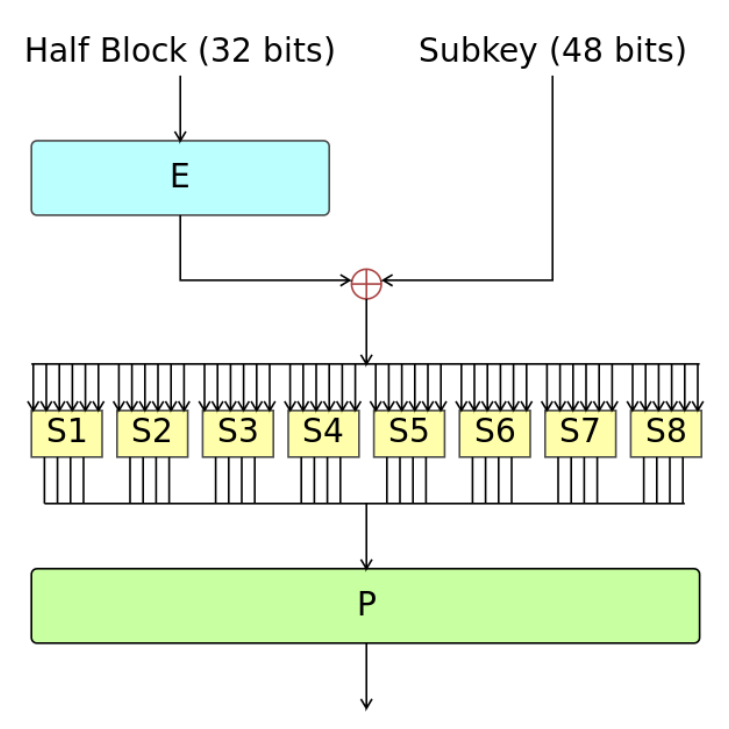
\includegraphics[width=220pt]{img/symmetric_cryptosystems/des_f_function}
    \caption{DES $f$ function}
  \end{figure}
  \item For DES the size of the input and output is 64 bits and there are 16 rounds
  \item The function $f$ for DES does the following on an input of a 32-bit data block $R$ and a round key $K$
  \begin{equation*}
    f(R,K) = P(S(K \oplus E(R)))
  \end{equation*}
  \item For functions $E$, $S$, $P$:
  \begin{itemize}
  	\item $E(R)$ is 48 bits long and contains the 32 bits of $R$ in a permuted order specified in the standard and 16 of the bits appear twice in the output
  	\item $S()$ takes as input 48 bits and returns 32 bits
    \begin{itemize}
  		\item It splits its input in 8 blocks $X_1, \dots X_8$ of 6 bits each
  		\item Then it computes $S_i(X_i)$ for $i=1, \dots,8$
  		\item Each $S_i$ is a function that takes 6 bits to 4 bits
  		\item The functions $S_i$ are known as substitution boxes or S-boxes
  		\item The functions are specified by tables that list for each input what the output should be
  		\item The output is $S(X) = S_1(X_1) \mid \mid \dots \mid \mid S_8(X_8)$
    \end{itemize}
  	\item $P()$ is a permutation that takes 32 bits as input and returns 32 bits
    \begin{itemize}
  		\item It outputs the input bits in a permuted order that is fixed in the standard
    \end{itemize}
  \end{itemize}

  \item S boxes are the heart of the security of DES
  \begin{itemize}
  	\item This is due to them being non-linear function
  	\item They have been chosen such that if one bit is flipped of the 6 inputs then at least 2 of the 4 output bits will change
    \begin{itemize}
  		\item This means similar strings $M$ and $M'$ will look random and unrelated
    \end{itemize}
  \end{itemize}
  \item The reason the function $E$ expands from 32 to 48 bits is to make it harder for an adversary to make a change such that only 1 S-box is affected
\end{itemize}

\subsection{Security definition}
\begin{itemize}
  \item Consider a family of functions $\{f_K \mid K \in \{0,1\}^K\}$ where each $f_k$ is a function $f_k : \{0,1\}^n \to \{0,1\}^m$
  \item A probabilistic algorithm $A$ (the adversary) is considered. It is placed in one of the following two scenarios and is asked which one it is in:
  \begin{itemize}
  	\item \textbf{The ideal world:} $A$ gets access to an oracle $O_{\text{Ideal}}$
    \begin{itemize}
  		\item Initially it chooses a random mapping $R$ from $\{0,1\}^n$ to $\{0,1\}^m$ uniformly
  		\item On input $x$, it answers with $R(x)$
    \end{itemize}
  	\item \textbf{The real world:} The adversary gets access to an oracle $O_\text{Real}$
    \begin{itemize}
  		\item Initially chooses $K$ at random from $\{0,1\}^k$
  		\item Fixes $K$ for the duration of the game
  		\item On input $x$ it answers with $f_K(x)$
    \end{itemize}
  \end{itemize}
  \item Consider a probabilistic algorithm $A$ that runs with access to either oracle $O_0$ or $O_1$ in the end $A$ should output a bit which the guess of which oracle he is talking to
  \begin{itemize}
  	\item Let $p(A,0)$ be the probability that $A$ outputs $1$ when talking to $O_o$
  	\item Let $p(A,1)$ be the probability that $A$ outputs $1$ when talking to $O_1$
  	\item The \textbf{advantage} of $A$ in distinguishing $O_0$ from $O_1$ is defined to be
    \begin{equation*}
      \text{Adv}_A(O_0,O_1) = |p(A,0) - p(A,1)|
    \end{equation*}
    \begin{itemize}
      \item If the advantage is small $\approx 0$ it implies that $A$ has no idea which case he is in
      \item If the advantage is large $\approx 1$ it implies that $A$ from $A's$ answers one can almost infer which case he was in
    \end{itemize}
  \end{itemize}
  \item \textbf{Definition 5.1 (PRF security)} $\{f_K \mid K \in \{0,1\}^k\}$ is a $(t,q, \epsilon)$ secure \textbf{psudorandom function family} (PRF), if any adversary $A$ that runs in time at most $t$ and makes at most $q$ calls to the oracle, satisfies $\text{Adv}_A(O_\text{Real}, O_\text{Ideal}) \leq \epsilon$

  \item To model security an encryption scheme using random encryption, a cryptosystem $(G,E,D)$ and an adversary $A$ is considered and placed in one of the following two scenarios where he has to guess which scenario he is in:
  \begin{itemize}
  	\item \textbf{The ideal world:} $A$ gets access to an oracle $O_\text{Ideal}$ which on input $x$ answers with $E_K(r)$
    \begin{itemize}
  		\item Where $r$ is a randomly chosen message where $|x| = |r|$
  		\item The $K$ is produced by $G$ but fixed in the entire attack
    \end{itemize}
  	\item \textbf{The real world:} $A$ gets access to normal chosen message attack
  \end{itemize}
  \item \textbf{Definition 5.2 (Chosen-Plaintext Attack(CPA)-security)} The cryptosystem $(G,E,D)$ is $(t,q, \mu, \epsilon)$ secure, if any adversary $A$ that runs in $t$ time, makes at most $q$ calls to the oracle and with plaintexts consisting of total of $\mu$ bits, it holds that $\text{Adv}_A(O_\text{Real}, O_\text{Ideal}) \leq \epsilon$
\end{itemize}

\subsection{Symmetric Encryption from Psudorandom Functions}
\subsubsection{CBC Encryption}
\begin{itemize}
  \item Let a block cipher be given $(G',E',D')$ where $\mathcal P = \mathcal C = \{0,1\}^n$ for some $n$
  \item CBC encryption is a way to make a cryptosystem $(G,E,D)$ from the PRF defined by the block cipher $(G',E',D')$
  \begin{itemize}
  	\item It sets $G' = G$
  	\item The plaintext set for the new system will be all strings of length divisible by $n$
  	\item Encryption is done by
    \begin{itemize}
  		\item Choosing a random $n$ bit string $y_0$
  		\item Split the input $x$ into $n$ bit strings $x_1,\dots,x_t$
  		\item Define for $i>0$ that $y_i = E_K(y_{i-1} \oplus x_i)$
  		\item The output ciphertext is $y_0,y_1,\dots,y_t$
    \end{itemize}
  	\item Decryption is straightforward
  \end{itemize}

  \item \textbf{Theorem 5.3} Suppose $(G',E',D')$ is a $(t',q', \epsilon')$ secure PRF. Then CBC encryption based on this system is CPA $(t,q,\mu,\epsilon)$ secure for any $q$, and for
  \begin{equation*}
    \epsilon = \epsilon + \bigg(\frac{\mu}n\bigg)^2 \cdot \frac1{2^n}
  \end{equation*}
  provided that
  \begin{equation*}
    t \leq t', \quad \frac\mu{n} \leq q'
  \end{equation*}
  \textbf{Proof}
  \begin{itemize}
  	\item A new game called \textbf{hybrid} is introduced
    \begin{itemize}
    	\item It chooses a random function $R$ from $n$ bits to $n$ bits 
      \item On input some message $m$ from the adversary ``encrypts'' $m$ using CBC mode but where the block cipher is replaced by $R$
    \end{itemize} 
    \item $p(A, \text{hybrid})$ is defined to be the probability that $A$ outputs $1$ when playing the hybrid game
    \item $p(A, ideal)$, $p(A, real)$ are the probabilities of output $1$ when $A$ talks to $O_{ideal}$ or $O_{real}$ respectively
    \item Since the only difference between the idea and the real game is that $R()$ is replaced by $E_k()$ and thus it must be the case that 
    \begin{equation*}
      |p(A, real) - p(A, hybrid) | \leq \epsilon '
    \end{equation*}
    \item The ideal game is completely equivalent to a game where the Oracle on input an $N$-block message always returns a randomly chosen sequence of $N+1$ blocks
    \begin{itemize}
    	\item The hybrid games also does this with high probability
    \end{itemize}
    \item Define the event BAD as follows: BAD occurs, if at any point during the hybrid game, the function $R$ receives an input that it has received before in this game
    \begin{itemize}
    	\item If BAD does not occur then since $R$ is a random function all outputs generated by $R$ will be random blocks chosen independently of everything else.
      \item The output generated will be completely random as in the ideal case
    \end{itemize}
    \item The only change of telling the ideal and the hybrid game apart is if BAD occurs i.e.
    \[
      |p(A,hybrid) - p(A,ideal) \leq \Pr(\text{BAD})
    \]
    Together with $|p(A,real) - p(A, hybrid) | \leq \epsilon'$ it implies
    \[
      Adv_A(O_{real}, O_{ideal}) = |p(A,real) - p(A,ideal) | \leq \epsilon' + \Pr(\text{BAD})
    \]
    Thus the last thing needed to be estimated is $\Pr(\text{BAD})$ 
    \item Let $M_j$ be the event that a collision occurs after $j$ calls to $R$
    \item Clearly $P(M_1) = 0$ 
    \item It must be the case using the standard formula for conditional probabilities that 
    \begin{equation*}
      P(M_j) \leq P(M_{j-1}) + P(M_J | \not M_{j-1})
    \end{equation*}
    \item $P(M_J | \neg M_{j-1}) = (j-1)/2^{n}$ since 
    \begin{itemize}
      \item $M_{j-1}$ did not occur there must have been $j-1$ different inputs before 
      \item The jth input is the XOR of some message block and an independently chosen random block and is therefore uniformly chosen
    \end{itemize}
    \item Thereby it must be the case that
    \begin{equation*}
      P(M_j) \leq (1+2+\cdots + (j-1))/ 2^n \leq j^2/2^n
    \end{equation*}
    Since the total number of calls is at most $\mu /n$ is follows that 
    \begin{equation*}
      \Pr(\text{BAD}) \leq \frac{\mu^2}{n^22^n}
    \end{equation*}
  \end{itemize}

\end{itemize}

\subsubsection{Counter (CTR) Mode}
\begin{itemize}
  \item The construction is the same form as CBC encryption, the only difference is the encryption algorithm is as follows:
  \begin{itemize}
  	\item Chooses a random $n$ bit string $y_0$
  	\item Split $x$ into $n$ bit strings $x_1, \dots, x_t$
  	\item Define for $i>0$ that $y_i = E_k(y_0+i) \oplus x_i$
  	\item Here $y_0 +i$ means that $i$ is written in binary and addition is done modulo $2^n$
  \end{itemize}

  \item \textbf{Theorem 5.4} Suppose $(G',E',D')$ is $(t',q',\epsilon')$ secure PRF. Then Counter mode based on this system is CPA $(t,q,\mu,\epsilon)$ secure for any $q$ and where
  \begin{equation*}
    t \leq t' \quad \frac{mu}{n} \leq q' \quad \epsilon = \epsilon' + \bigg(\frac{\mu}{n}\bigg)^n \cdot \frac1{2^n}
  \end{equation*}
  \textbf{Proof}
  \begin{itemize}
  	\item A game called Hybrid is defined as in the proof for Theorem 5.3
    \item As in the Theorem 5.3 proof an event BAD is defined and thus using similar reasoning as in Theorem 5.3 the advantage is bounded by $\Pr(\text{BAD})$
    \item Let $B_j$ denote the probability that any of the blocks used as input to $R$ during the jth call to the oracle collide with blocks used in other calls
    \item Let $b_j$ denote the number of blocks encrypted during the jth call 
    \item Consider a single block input to $R$ during the $j$'th call
    \begin{itemize}
    	\item The block is of the form $y_0 + i$ for some $i$ 
      \item It is uniformly chosen since $y_0$ is uniform
      \item It is chosen independently of all blocks used in other calls
    \end{itemize}
    \item There are at most $\mu / n$ other blocks so the probability the probability that $y_0 + i$ collides with any of these it as most $\frac{\mu}{n2^n}$
    \begin{itemize}
    	\item By the union bound it must be the case that $\Pr(B_j) \leq \frac{b_j \mu}{n 2^n}$
    \end{itemize}
    \item BAD occurs if at least one $B_j$s must occur, so by the union bound and because the total number of blocks encrypted is $\mu/n$, we have
    \[
      \Pr(\text{BAD}) \leq \sum_{j=1}^q P(B_j) = \frac{\mu}{n2^n} \sum_{j=1}^n b_j = \left(\frac{\mu}{n}\right)^2 \cdot \frac1{2^n}
    \]
  which proves the theorem
  \end{itemize}
\end{itemize}

\newpage

%%% Local Variables:
%%% mode: latex
%%% TeX-master: "crypto-noter"
%%% End:
